\documentclass[aspectratio=169]{beamer}

\usetheme{durham}

\usepackage{booktabs}
\usepackage{array}
\usepackage{hyperref}
\usepackage{graphicx}
\usepackage{tikz}
\usetikzlibrary{arrows.meta,positioning}

\title[Filipino OmniVoice Fine-Tuning]{Low-Resource Filipino Adaptation of OmniVoice for Voice Cloning and Text-to-Speech}
\subtitle{Research Project Proposal}
\author{}
\institute{Current Trends}
\date{\today}
\setbeamertemplate{footline}{}

\begin{document}

\maketitle

\begin{frame}{Research Problem}
  Voice cloning is an emerging AI technology that can synthesize speech in a target speaker's voice from a short reference audio.

  \vspace{0.6em}

  \begin{itemize}
    \item Most high-quality voice cloning systems are strongest in high-resource languages.
    \item Filipino speech AI remains relatively low-resource.
    \item There are few open, Filipino-focused voice cloning workflows.
    \item A practical opportunity is adapting an existing multilingual model instead of training from scratch.
  \end{itemize}
\end{frame}

\begin{frame}{Motivation}
  \begin{itemize}
    \item Filipino voice cloning can support education, accessibility, narration, localization, and language learning tools.
    \item Multilingual TTS models report wide language coverage, but quality can still vary across low-resource languages.
    \item OmniVoice supports Filipino, but its language table lists only about \textbf{7.71 hours} of Filipino in the training mixture.
  \end{itemize}

  \vspace{0.7em}

  \begin{block}{Research Opportunity}
    Evaluate whether curated Filipino speech can improve a pretrained multilingual voice cloning model.
  \end{block}
\end{frame}

\begin{frame}{Background: OmniVoice}
  \begin{columns}[T]
    \begin{column}{0.38\textwidth}
      
\includegraphics[height=0.66\textheight,keepaspectratio]{\detokenize{../../images/omnivoice paper.png}}
    \end{column}
    \begin{column}{0.58\textwidth}
      \begin{itemize}
        \item Open-source multilingual zero-shot TTS and voice cloning model.
        \item Supports 600+ languages, including Filipino.
        \item Uses a diffusion language model-style masked-token generation approach.
        \item Supports voice cloning, voice design, and automatic voice generation.
        \item Provides official fine-tuning scripts.
      \end{itemize}
      \vspace{0.5em}
      \small Source: Zhu et al. (2026).
    \end{column}
  \end{columns}
\end{frame}

\begin{frame}{Filipino Coverage in OmniVoice}
  \begin{columns}[T]
    \begin{column}{0.45\textwidth}
      
\includegraphics[height=0.66\textheight,keepaspectratio]{\detokenize{../../images/omnivoice filipino dataset.png}}
    \end{column}
    \begin{column}{0.50\textwidth}
      \begin{itemize}
        \item OmniVoice reports 646 supported languages and 581k hours of total training data.
        \item Filipino is included with language ID \texttt{fil}.
        \item Filipino has about \textbf{7.71 hours} in the OmniVoice training mixture.
      \end{itemize}

      \vspace{0.5em}
      \begin{block}{Research Angle}
        Filipino exists in the base model, but the available Filipino training hours are low compared with major languages.
      \end{block}
    \end{column}
  \end{columns}
\end{frame}

\begin{frame}{Research Question and Scope}
  \begin{block}{Main Research Question}
    How much does Filipino-specific fine-tuning improve OmniVoice performance for Filipino TTS and voice cloning across intelligibility, naturalness, and speaker similarity metrics?
  \end{block}

  \vspace{0.5em}

  \begin{itemize}
    \item Model: \texttt{k2-fsa/OmniVoice}
    \item Language: Filipino (\texttt{fil})
    \item Dataset: Filipino subset of UP-DSP Philippine Languages Database
    \item Method: fine-tuning, not training from scratch
    \item Output: generated samples and evaluation after implementation
    \item Baseline: measure change against the base OmniVoice checkpoint
  \end{itemize}
\end{frame}

\begin{frame}{Objectives}
  \begin{enumerate}
    \item Prepare a clean Filipino speech-text dataset for OmniVoice fine-tuning.
    \item Fine-tune the pretrained OmniVoice checkpoint on Filipino read speech.
    \item Generate Filipino speech using both base and fine-tuned models.
    \item Evaluate intelligibility, naturalness, and speaker similarity.
    \item Produce a reproducible workflow and demo samples for the existing voice cloning app.
  \end{enumerate}
\end{frame}

\begin{frame}{Related Work}
  \begin{itemize}
    \item \textbf{VALL-E / Neural Codec Language Models}: zero-shot TTS with discrete speech tokens.
    \item \textbf{Voicebox}: text-guided multilingual speech generation at scale.
    \item \textbf{F5-TTS and E2 TTS}: efficient non-autoregressive zero-shot TTS with flow matching.
    \item \textbf{MaskGCT}: masked generative codec modeling for zero-shot TTS.
    \item \textbf{OmniVoice}: extends multilingual zero-shot TTS toward 600+ languages.
    \item \textbf{UP-DSP PLD}: Filipino and Philippine-language data for low-resource speech systems.
  \end{itemize}
\end{frame}

\begin{frame}{Dataset}
  \textbf{UP-DSP Philippine Languages Database}

  \begin{columns}[T]
    \begin{column}{0.52\textwidth}
      
\includegraphics[width=\linewidth,height=0.60\textheight,keepaspectratio]{\detokenize{../../images/up dsp philippine languages database.png}}
    \end{column}
    \begin{column}{0.44\textwidth}
      \begin{itemize}
        \item Released through Mozilla Data Collective
        \item WAV audio with LOG transcript files
        \item License: CC-BY-NC-4.0
        \item Research use only; not for commercial deployment
      \end{itemize}
      \vspace{0.5em}
      \small Source: UP EEEI - DSP Laboratory (2026).
    \end{column}
  \end{columns}
\end{frame}

\begin{frame}{Filipino Dataset Statistics}
  \begin{columns}[T]
    \begin{column}{0.48\textwidth}
      
\includegraphics[height=0.66\textheight,keepaspectratio]{\detokenize{../../images/philippine languages database paper list of language.png}}
    \end{column}
    \begin{column}{0.48\textwidth}
      \begin{table}
        \centering
        \small
        \begin{tabular}{ll}
          \toprule
          Filipino subset & Value \\
          \midrule
          Language ID & \texttt{fil} \\
          Speakers & 135 \\
          Utterances & 52,879 \\
          Duration & 48:56:36 \\
          Avg. utterance length & 3.58 seconds \\
          \bottomrule
        \end{tabular}
      \end{table}
      \small Enough for a small fine-tuning study while staying feasible on Kaggle.

      \vspace{0.5em}
      \small Source: Guevara et al. (2024).
    \end{column}
  \end{columns}
\end{frame}

\begin{frame}{Data Choice}
  \begin{columns}[T]
    \begin{column}{0.48\textwidth}
      \textbf{Read Speech}
      \begin{itemize}
        \item Speaker reads a prepared prompt.
        \item Transcript matches the spoken sentence.
        \item Best first subset for TTS fine-tuning.
      \end{itemize}
    \end{column}
    \begin{column}{0.48\textwidth}
      \textbf{Spontaneous Speech}
      \begin{itemize}
        \item Speaker answers freely.
        \item Prompt may not be the transcript.
        \item Requires transcript verification.
      \end{itemize}
    \end{column}
  \end{columns}

  \vspace{0.7em}
  \begin{block}{Project Decision}
    Use Filipino read speech first to reduce transcript-audio mismatch.
  \end{block}
\end{frame}

\begin{frame}{OmniVoice Architecture}
  \begin{enumerate}
    \item Text is encoded with a language-model tokenizer.
    \item Reference audio is converted into discrete acoustic tokens.
    \item The model receives text, language tags, and optional reference voice tokens.
    \item During training, some acoustic tokens are masked.
    \item The model learns to reconstruct the masked tokens.
    \item During inference, generated tokens are decoded into speech audio.
  \end{enumerate}

  \vspace{0.5em}
  \begin{block}{Fine-Tuning Goal}
    Adapt the text-to-acoustic-token mapping toward Filipino speech patterns.
  \end{block}
\end{frame}

\begin{frame}{Proposed Fine-Tuning Pipeline}
  \centering
  \scriptsize
  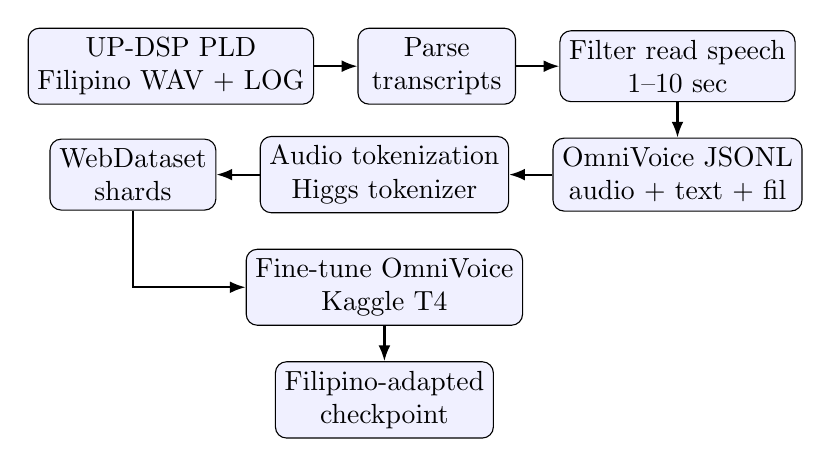
\begin{tikzpicture}[
    node distance=0.45cm and 0.55cm,
    box/.style={draw, rounded corners, align=center, minimum height=0.8cm, minimum width=2.0cm, fill=blue!6},
    arrow/.style={-{Latex[length=2mm]}, thick}
  ]
    \node[box] (a) {UP-DSP PLD\\Filipino WAV + LOG};
    \node[box, right=of a] (b) {Parse\\transcripts};
    \node[box, right=of b] (c) {Filter read speech\\1--10 sec};
    \node[box, below=of c] (d) {OmniVoice JSONL\\audio + text + fil};
    \node[box, left=of d] (e) {Audio tokenization\\Higgs tokenizer};
    \node[box, left=of e] (f) {WebDataset\\shards};
    \node[box, below=of e] (g) {Fine-tune OmniVoice\\Kaggle T4};
    \node[box, below=of g] (h) {Filipino-adapted\\checkpoint};

    \draw[arrow] (a) -- (b);
    \draw[arrow] (b) -- (c);
    \draw[arrow] (c) -- (d);
    \draw[arrow] (d) -- (e);
    \draw[arrow] (e) -- (f);
    \draw[arrow] (f) |- (g);
    \draw[arrow] (g) -- (h);
  \end{tikzpicture}
\end{frame}

\begin{frame}{Methodology}
  \begin{enumerate}
    \item Acquire the Filipino PLD subset.
    \item Parse WAV and LOG files into OmniVoice JSONL format.
    \item Filter clean read speech clips between 1 and 10 seconds.
    \item Split into train, development, and test sets.
    \item Tokenize audio using the OmniVoice audio tokenizer.
    \item Fine-tune \texttt{k2-fsa/OmniVoice} on Kaggle T4 GPUs.
    \item Generate matched test samples from base and fine-tuned models.
    \item Compare outputs using metrics and listener evaluation.
  \end{enumerate}
\end{frame}

\begin{frame}{Evaluation Design}
  \centering
  \scriptsize
  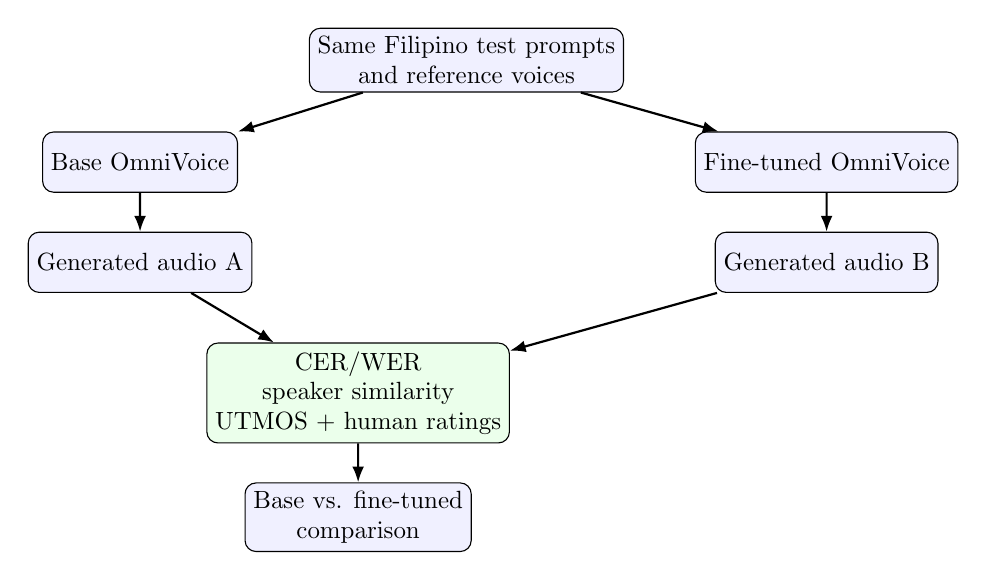
\begin{tikzpicture}[
    scale=0.90,
    transform shape,
    node distance=0.55cm and 1.0cm,
    box/.style={draw, rounded corners, align=center, minimum height=0.85cm, minimum width=2.4cm, fill=blue!6},
    metric/.style={draw, rounded corners, align=center, minimum height=0.85cm, minimum width=3.0cm, fill=green!8},
    arrow/.style={-{Latex[length=2mm]}, thick}
  ]
    \node[box] (t) {Same Filipino test prompts\\and reference voices};
    \node[box, below left=of t] (b) {Base OmniVoice};
    \node[box, below right=of t] (f) {Fine-tuned OmniVoice};
    \node[box, below=of b] (bo) {Generated audio A};
    \node[box, below=of f] (fo) {Generated audio B};
    \node[metric, below right=0.7cm and -0.65cm of bo] (m) {CER/WER\\speaker similarity\\UTMOS + human ratings};
    \node[box, below=of m] (r) {Base vs. fine-tuned\\comparison};

    \draw[arrow] (t) -- (b);
    \draw[arrow] (t) -- (f);
    \draw[arrow] (b) -- (bo);
    \draw[arrow] (f) -- (fo);
    \draw[arrow] (bo) -- (m);
    \draw[arrow] (fo) -- (m);
    \draw[arrow] (m) -- (r);
  \end{tikzpicture}
\end{frame}

\begin{frame}{Fine-Tuning Setup}
  \begin{itemize}
    \item Environment: Kaggle notebook with 2x NVIDIA T4 GPUs.
    \item Tools: PyTorch, Hugging Face Transformers, Accelerate, DeepSpeed.
  \end{itemize}

  \vspace{0.5em}

  \begin{table}
    \centering
    \small
    \begin{tabular}{ll}
      \toprule
      Setting & Planned value \\
      \midrule
      Starting checkpoint & \texttt{k2-fsa/OmniVoice} \\
      Data size & 5--10 hours clean read speech \\
      Precision & FP16 \\
      Attention & SDPA \\
      Learning rate & 5e-6 \\
      Steps & 1,000--2,000 \\
      Optimization & DeepSpeed ZeRO-2 \\
      \bottomrule
    \end{tabular}
  \end{table}
\end{frame}

\begin{frame}{Model Testing and Metrics}
  \begin{table}
    \centering
    \small
    \begin{tabular}{p{0.30\textwidth}p{0.55\textwidth}}
      \toprule
      System & Description \\
      \midrule
      Base OmniVoice & Original pretrained checkpoint \\
      Fine-tuned OmniVoice & Adapted using Filipino read speech \\
      \bottomrule
    \end{tabular}
  \end{table}

  \vspace{0.4em}

  \begin{itemize}
    \item \textbf{CER/WER}: ASR transcript vs. target text.
    \item \textbf{Speaker similarity}: reference vs. generated voice embeddings.
    \item \textbf{UTMOS}: predicted naturalness, if feasible.
    \item \textbf{Human ratings}: pronunciation, naturalness, intelligibility, speaker similarity, preference.
  \end{itemize}

  \vspace{0.3em}
  \small OmniVoice uses the same metric families: WER/CER, SIM-o, UTMOS, CMOS, and SMOS.
\end{frame}

\begin{frame}{How the Metrics Work}
  \begin{itemize}
    \item \textbf{CER/WER: ``Did it say the right words?''}\\
    ASR transcribes generated audio; the transcript is compared with the target text. Lower is better.
    \item \textbf{Speaker similarity: ``Does it sound like the reference?''}\\
    Speaker embeddings from reference and generated audio are compared. Higher is better.
    \item \textbf{UTMOS: ``Does it sound natural?''}\\
    A prediction model estimates naturalness from the generated waveform. Higher is better.
    \item \textbf{Human ratings: ``Which sounds better to Filipino listeners?''}\\
    Raters judge pronunciation, naturalness, intelligibility, similarity, and preference.
  \end{itemize}
\end{frame}

\begin{frame}{Expected Contribution}
  \begin{itemize}
    \item Practical Filipino OmniVoice fine-tuning workflow.
    \item Cleaned Filipino JSONL manifests and experiment setup.
    \item Base-vs-fine-tuned comparison using measurable metrics.
    \item Generated audio samples for the existing voice cloning application.
    \item Evidence on whether low-resource Filipino adaptation is feasible under limited compute.
  \end{itemize}
\end{frame}

\begin{frame}{Application Use Case: Voice Cloning}
  \centering
  
\includegraphics[width=0.94\linewidth,height=0.78\textheight,keepaspectratio]{\detokenize{../../images/app 1.png}}
\end{frame}

\begin{frame}{Application Use Case: Speech Generation}
  \centering
  
\includegraphics[width=0.94\linewidth,height=0.78\textheight,keepaspectratio]{\detokenize{../../images/app 2.png}}
\end{frame}

\begin{frame}{Application Use Case: Clone Workflow}
  \centering
  
\includegraphics[width=0.94\linewidth,height=0.78\textheight,keepaspectratio]{\detokenize{../../images/app 3.png}}
\end{frame}

\begin{frame}{References}
  \tiny
  \begin{itemize}
    \item Chen, S., Wang, C., Wu, Y., Zhang, Z., Zhou, L., Liu, S., Chen, Z., Liu, Y., Wang, H., Li, J., et al. (2025). \textit{Neural codec language models are zero-shot text to speech synthesizers}. IEEE/ACM Transactions on Audio, Speech, and Language Processing.
    \item Chen, Y., Niu, Z., Ma, Z., Deng, K., Wang, C., Zhao, J., Yu, K., \& Chen, X. (2024). \textit{F5-TTS: A fairytaler that fakes fluent and faithful speech with flow matching}. arXiv. \url{https://arxiv.org/abs/2410.06885}
    \item Guevara, R. C. L., Cajote, R. D., Bayona, M. G. A. R., \& Lucas, C. R. G. (2024). \textit{Philippine Languages Database: A multilingual speech corpora for developing systems for low-resource languages}. SIGUL 2024. \url{https://aclanthology.org/2024.sigul-1.32/}
    \item Le, M., Vyas, A., Shi, B., Karrer, B., Sari, L., Moritz, R., Williamson, M., Manohar, V., Adi, Y., Mahadeokar, J., et al. (2023). \textit{Voicebox: Text-guided multilingual universal speech generation at scale}. NeurIPS, 36, 14005--14034.
    \item UP EEEI - Digital Signal Processing Laboratory. (2026). \textit{UP-DSP Philippine Languages Database}. Mozilla Data Collective. \url{https://mozilladatacollective.com/datasets/cmmxhw46c00tqnw07xyr94zjk}
    \item Wang, Y., Zhan, H., Liu, L., Zeng, R., Guo, H., Zheng, J., Zhang, Q., Zhang, X., Zhang, S., \& Wu, Z. (2025). \textit{MaskGCT: Zero-shot text-to-speech with masked generative codec transformer}. ICLR.
    \item Zhu, H., Ye, L., Kang, W., Yao, Z., Guo, L., Kuang, F., Han, Z., Zhuang, W., Lin, L., \& Povey, D. (2026). \textit{OmniVoice: Towards omnilingual zero-shot text-to-speech with diffusion language models}. arXiv. \url{https://arxiv.org/abs/2604.00688}
  \end{itemize}
\end{frame}

\end{document}
